\documentclass[fleqn, 12pt]{article}
\usepackage[utf8]{inputenc} % default from sharelatex
\usepackage[a4paper, left=30mm, right=30mm, top=30mm, bottom=30mm]{geometry}
\usepackage{indentfirst} % to indent fist paragraph
\usepackage[brazilian]{babel} % BR
\usepackage{amsmath}
\usepackage{graphicx} % to have pictures

\graphicspath{{images/}}

\title{Teoria dos números e corpos finitos}

\author{Lucas João Martins}
\date{}

\begin{document}

\maketitle

\section*{}
\subsection*{1. (4.6) For each of the following equations, find an integer $x$
that satisfies the equation.}
  \subsubsection*{a. $5x \equiv 4 \ \ (mod \ \ 3)$}
    \begin{align*}
      & x = 2 \\
      & 5 \times 2 = 10 \\
      & 10 - 4 = 6 = 3 \times 2
    \end{align*}
  \subsubsection*{b. $7x \equiv 6 \ \ (mod \ \ 5)$}
    \begin{align*}
      & x = 3 \\
      & 7 \times 3 = 21 \\
      & 21 - 6 = 15 = 5 \times 3
    \end{align*}
  \subsubsection*{c. $9x \equiv 8 \ \ (mod \ \ 7)$}
    \begin{align*}
      & x = 4 \\
      & 9 \times 4 = 36 \\
      & 36 - 8 = 28 = 7 \times 4
    \end{align*}

\subsection*{2. (4.7) In this text, we assume that the modulus is a positive
integer. But the definition of the expression $a \ \ mod \ \ n$ also makes
 perfect sense if $n$ is negative. Determine the following:}

  Usando $a \ \ mod \ \ n = a - \lfloor a / n \rfloor \times n$.

  \subsubsection*{a. $5 \ \ mod \ \ 3$}
    \begin{align*}
      & 2
    \end{align*}
  \subsubsection*{b. $5 \ \ mod \ \ -3$}
    \begin{align*}
      & 5 - \lfloor 5 / -3 \rfloor \times -3 \\
      & 5 - (-2 \times -3) \\
      & 5 - 6 \\
      & -1 \\
    \end{align*}
  \subsubsection*{c.  $-5 \ \ mod \ \ 3$}
    \begin{align*}
      & -5 - \lfloor -5 / 3 \rfloor \times 3 \\
      & -5 - (-2 \times 3) \\
      & -5 + 6 \\
      & 1 \\
    \end{align*}
  \subsubsection*{d. $-5 \ \ mod \ \ -3$}
    \begin{align*}
      & -5 - \lfloor -5 / -3 \rfloor \times -3 \\
      & -5 - (1 \times -3) \\
      & -5 + 3 \\
      & -2 \\
    \end{align*}

\subsection*{3. (4.8) A modulus of 0 does not fit the definition but is defined
by convention as follows: $a \ \ mod \ \ 0 = a$. With this definition in mind,
what does the following expression mean: $a \equiv b \ \ (mod \ \ 0)$?}

  Significa que $a$ e $b$ são iguais.

\subsection*{4. (4.1) For the group $S_n$ of all permutations of $n$ distinct
symbols:}
  \subsubsection*{a. what is the number of elements in $S_n$?}

    $n!$

  \subsubsection*{b. show that $S_n$ is not abelian for $n > 2$.}

    Um contra exemplo com o $S_3$ seria:

    \begin{align*}
      & \lbrace 3, 2, 1 \rbrace \cdot \lbrace 1, 3, 2 \rbrace = \lbrace 2, 3, 1
      \rbrace \\
      & \lbrace 1, 3, 2 \rbrace \cdot \lbrace 3, 2, 1 \rbrace = \lbrace 3, 1, 2
      \rbrace \\
    \end{align*}

\subsection*{5. (4.4) Reformulate Equation (4.1), removing the restriction that
$a$ is a nonnegative integer. That is, let a be any integer.}

    A equação continua a mesma.

\subsection*{6. (4.5) Draw a figure similar to Figure 4.1 for $a < 0$.}
  \begin{figure}[h]
    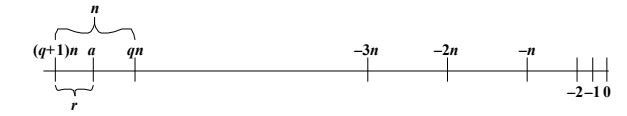
\includegraphics[width=\linewidth]{quatro_seis}
  \end{figure}

\subsection*{7. (4.13) Find the multiplicative inverse of each nonzero element
in $Z_5$.}

    Para todo $a \in Z_5$, precisamos encontrar um $b \in Z_5$ onde $ab \equiv 1
    \ \ (mod \ \ 5)$

    \begin{align*}
      & 1 \rightarrow 1 \\
      & 2 \rightarrow 3 \\
      & 3 \rightarrow 2 \\
      & 4 \rightarrow 4 \\
    \end{align*}

\subsection*{8. (4.20) Develop a set of tables similar to Table 4.3 for GF(5).}
  \begin{figure}[h]
    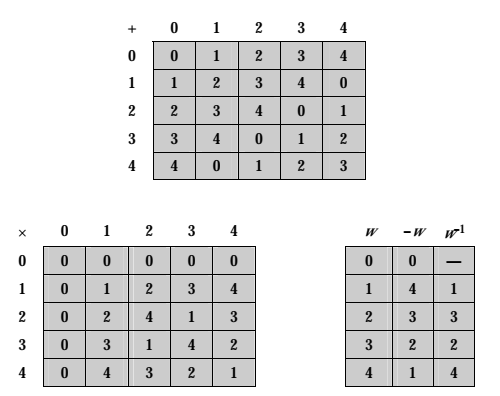
\includegraphics[width=\linewidth]{quatro_vinte}
  \end{figure}

\subsection*{9. (4.10) What is the smallest positive integer that has exactly k
divisors, for $1 \leq k \leq 6$?}
  \begin{align*}
    & k = 1 \rightarrow 1 \rightarrow \lbrace 1 \rbrace \\
    & k = 2 \rightarrow 2 \rightarrow \lbrace 1, 2 \rbrace \\
    & k = 3 \rightarrow 4 \rightarrow \lbrace 1, 2, 4 \rbrace \\
    & k = 4 \rightarrow 6 \rightarrow \lbrace 1, 2, 3, 6 \rbrace \\
    & k = 5 \rightarrow 16 \rightarrow \lbrace 1, 2, 4, 8, 16 \rbrace \\
    & k = 6 \rightarrow 12 \rightarrow \lbrace 1, 2, 3, 4, 6, 12 \rbrace \\
  \end{align*}

\subsection*{10. (4.2) Does the set of residue classes (mod 3) form a group}

    Considere as seguintes tabelas de multiplicação e adição para responder as
    perguntas:

    \begin{table}[h]
      \centering
      \caption{Adição}
      \begin{tabular}{|c|c|c|c|}
      \hline
      + & 0 & 1 & 2  \\ \hline
      0 & 0 & 1 & 2  \\ \hline
      1 & 1 & 2 & 0  \\ \hline
      2 & 2 & 0 & 1  \\ \hline
      \end{tabular}
    \end{table}

    \begin{table}[h]
      \centering
      \caption{Multiplicação}
      \begin{tabular}{|c|c|c|c|}
      \hline
      x & 0 & 1 & 2  \\ \hline
      0 & 0 & 0 & 0  \\ \hline
      1 & 0 & 1 & 2  \\ \hline
      2 & 0 & 2 & 1  \\ \hline
      \end{tabular}
    \end{table}

  \subsubsection*{a. with respect to modular addition?}

    Sim, o elemento identidade é 0 e a inversa de 0, 1, 2 são respectivamente 0,
    2, 1.

  \subsubsection*{b. with respect to modular multiplication?}

    Não, o elemento identidade é 1, mas 0 não possui inversa.

\subsection*{11. (4.3) Consider the set $S = \lbrace a, b \rbrace$ with addition
and multiplication defined by the following tables. Is S a ring? Justify your
answer.}
  \begin{figure}[h]
    \centering
    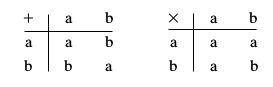
\includegraphics{quatro_tres}
  \end{figure}

  $S$ é um anel por causa dos seguintes motivos:
  \begin{itemize}
    \item a soma de qualquer dois elementos em $S$ resulta em um elemento também
    em $S$
    \item ele é associativo sobre a adição
    \item $a$ é a identidade da adição
    \item a inversa aditiva de $a$ e $b$ são $b$ e $a$ respectivamente
    \item ele é comutativo sobre a adição
    \item o produto de qualquer dois elementos em $S$ resulta em um elemento
    também em $S$
    \item ele é associativo sobre o produto
    \item ele é distributivo sobre as duas operações
  \end{itemize}

\subsection*{12. (4.11) Prove the following:}

  \subsubsection*{a. $a \equiv b \ \ (mod \ \ n)$ implies $b \equiv a \ \ (mod \
  \ n)$}

    Essa é a definição de congruência apresentada no livro.

  \subsubsection*{b. $a \equiv b \ \ (mod \ \ n)$ and $b \equiv c \ \ (mod \ \
  n)$ imply $a \equiv c \ \ (mod n)$}

    As duas primeiras significam:

    \begin{align*}
      & a - b = nk \\
      & b - c = nm \\
    \end{align*}

    Então substituindo:

    \begin{align*}
      & a - c = (a - b) + (b - c) = n (k + m)\\
    \end{align*}

\subsection*{13. (4.12) Prove the following:}

  \subsubsection*{a. $\lbrack (a \ \ mod \ \ n) - (b \ \ mod \ \ n ) \rbrack
  \ \ mod \ \ n \equiv (a - b) \ \ mod \ \ n$}

    Considere o seguinte:

    \begin{align*}
      & c = a \ \ mod \ \ n \\
      & d = b \ \ mod \ \ n \\
    \end{align*}

    Então:

    \begin{align*}
      & c = a + kn \\
      & d = b + mn \\
      & c - d = (a - b) + (k - m) \times n \\
      & (c - d) = (a - b) \ \ mod \ \ n
    \end{align*}

  \subsubsection*{b. $\lbrack (a \ \ mod \ \ n) \times (b \ \ mod \ \ n )
  \rbrack \ \ mod \ \ n \equiv (a \times b) \ \ mod \ \ n$}

    Com as definições de $c$ e $d$ da alternativa anterior:

    \begin{align*}
      & cd = ab + n \times (kb + ma + kmn) \\
      & cd = (a \times b) \ \ mod \ \ n
    \end{align*}

\subsection*{14. (4.9) In Section 4.3, we define the congruence relationship as
follows: Two integers $a$ and $b$ are said to be congruent modulo $n$ if $(a \ \
mod \ \ n) = (b \ \ mod \ \ n)$. We then proved that $a \equiv b (mod \ \ n)$ if
$n | (a - b)$. Some texts on number theory use this latter relationship as the
definition of congruence: Two integers $a$ and $b$ are said to be congruent
modulo $n$ if $n | (a - b)$. Using this latter definition as the starting point,
prove that, if $(a \ \  mod \ \ n) = (b \ \ mod \ \ n)$, then $n$ divides $(a -
b)$.}

    Qualquer inteiro $a$ pode ser escrito como $a = qn + r$ onde $q$ é algum
    inteiro e $r$ é um número entre $0, 1, 2, \dots, n - 1$. Usando a segunda
    definição, não há dois restos na lista citada que são congruente módulo $n$,
    porque a diferença entre eles é menor que $n$ e portando $n$ não divide essa
    diferença. Portando, esses dois números devem ter restos diferentes. Então é
    possível concluir que $n$ divide $(a - b)$ se e somente se $a$ e $b$ são
    números que possuem o mesmo resto quando dividido por $n$.

\subsection*{15. (4.14) Show that an integer $N$ is congruent modulo 9 to the
sum of its decimal digits. For example, $475 \equiv 4 + 7 + 5 \equiv 16 \equiv 1
+ 6 \equiv 7 \ \ (mod \ \ 9)$. This is the basis for the familiar procedure of
“casting out 9’s” when checking computations in arithmetic}

    Temos:

    \begin{align*}
      & 1 \equiv 1 (mod \ \ 9) \\
      & 10 \equiv 1 (mod \ \ 9) \\
      & 10^2 \equiv 10(10) \equiv 1(1) (mod \ \ 9) \\
      & 10^{n-1} \equiv 1 (mod \ \ 9) \\
    \end{align*}

    Se escrever $N = a_0 + a_110^1 + \dots + a_{n-1}10^{n-1}$. Então $N \equiv
    a_0 + a_1 + \dots + a_{n-1} (mod \ \ 9)$.

\subsection*{16. (4.27) Determine the multiplicative inverse of $x^3 + x + 1$ in
GF($2^4$) with $m(x) = x^4 + x + 1$.}

    $x^2 + 1$

\subsection*{17. (4.28) Develop a table similar to Table 4.9 for GF($2^4$) with
$m(x) = x^4 + x + 1$.}
    \begin{figure}[h]
      \centering
      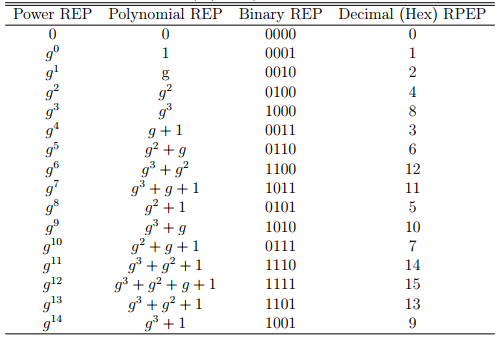
\includegraphics{quatro_vinte_e_oito}
    \end{figure}

\subsection*{18. (4.23) For polynomial arithmetic with coefficients in $Z_{10}$,
perform the following calculations.}

  \subsubsection*{a. $(7x + 2) - (x^2 + 5)$:}

    $9x^2 + 7x + 7$

  \subsubsection*{a. $(6x^2 + x + 3) \times (5x^2 + 2)$:}

    $5x^3 + 7x^2 + 2x + 6$

\subsection*{19. (4.22) Demonstrate whether each of these statements is true or
false for polynomials over a field.}

  \subsubsection*{a. The product of monic polynomials is monic.}

    True. O único termo que não é zero no resultado terá valor igual a 1.

  \subsubsection*{b. The product of polynomials of degrees $m$ and $n$ has
  degree $m + n$.}

    True. Temos $c_{n + m} = a_nb_m \neq 0$.

  \subsubsection*{c. The sum of polynomials of degrees $m$ and $n$ has degree
  $max \lbrack m, n \rbrack$.}

    True quando $m \ne n$, mas false no geral quando $m = n$, por causa que os
    coeficientes com maiores graus podem se cancelar.

\subsection*{20. (4.19) Using the extended Euclidean algorithm, find the
multiplicative inverse of}

  \subsubsection*{a. $1234 \ \ mod \ \ 4321$:}

    $1234$

  \subsubsection*{b. $1234 \ \ mod \ \ 4321$:}

    $gcd(40902, 24240) = 34 \ne 1$.

  \subsubsection*{c. $550 \ \ mod \ \ 1769$:}

    $550$

\end{document}
